\newcommand{\sidenote}[1]{\begin{itemize} \item #1 \end{itemize}}
\newcommand{\hlmath}[1]{\textrm{\color{blue}\ensuremath{#1}}}

\pgfdeclarelayer{bg}
\pgfsetlayers{bg,main}
\newcommand{\obj}[1]{%
    {%
    \begin{minipage}{6cm}
      #1
    \end{minipage}
    }
}
\newcommand{\objw}[2]{%
    {%
    \begin{minipage}{#1}
      #2
    \end{minipage}
    }
}
\tikzstyle{box}=[scale=0.8,rectangle,fill=white,draw=black]
\tikzstyle{loop}=[smooth,dashed,in=-90,out=-90,looseness=0.75]

\makeatletter
\newcommand*{\centerfloat}{%
  \parindent \z@
  \leftskip \z@ \@plus 1fil \@minus \textwidth
  \rightskip\leftskip
  \parfillskip \z@skip}
\makeatother

\newcommand*{\tikzgridon}{%
\setbeamertemplate{background canvas}{%
\begin{tikzpicture}[remember picture, overlay]
    \draw[help lines,xstep=.25,ystep=.25,gray!20] (current page.south west) grid (current page.north east);
    \draw[help lines,xstep=1,ystep=1,gray] (current page.south west) grid (current page.north east);
    \foreach \x in {-15,-14.5,...,15} {%
        \node [anchor=north, gray] at (\x,0) {\tiny \x};
        \node [anchor=east,gray] at (0,\x) {\tiny \x};
    }
\end{tikzpicture}
}
}
\newcommand{\tikzgridoff}{\setbeamertemplate{background canvas}{}}

% Input is dimensions
\newcommand*{\tikzrect}[4]{%
  \draw[#1] #2 -- ++(-#3,0) -- ++(0,-#4) -- ++(#3,0) -- cycle;
}

\newcommand*{\tikzcube}[5]{%
  \draw[#1] #2 -- ++(-#3,0,0) -- ++(0,-#4,0) -- ++(#3,0,0) -- cycle;
  \draw[#1] #2 -- ++(0,0,-#5) -- ++(0,-#4,0) -- ++(0,0,#5) -- cycle;
  \draw[#1] #2 -- ++(-#3,0,0) -- ++(0,0,-#5) -- ++(#3,0,0) -- cycle;
}
